\section{Collision detection\label{collisionDetection}}

\subsection{Intersection of triangle meshes\label{meshIntersection}}

Before any dynamic interaction between bodies can be tackled, a simulation needs to know which
meshes are geometrically in contact, and what type of contact is present. This is the subject
of collision detection. The simplest algorithm for this purpose would be to take each triangle
of one mesh and test it for intersection~\cite{Moeller:97} against each triangle of the other
mesh. This $O(N^2)$ algorithm is clearly very inefficient; most research in collision detection
endeavours to create algorithms which are as close as possible to $O(1)$ complexity, but
semantically equivalent.

Fast computation is only a minor concern in this project, therefore I shall describe my solution
only very briefly. This algorithm was suggested by Brett Saunders and is simpler than most
published algorithms, but still very effective.

For each mesh, the closest-fitting Axis-Aligned Bounding Box (AABB) is computed. The set of
triangles is split approximately in half along the axis of the longest bounding box side, and
an AABB is computed for each subset of triangles (the two new AABBs may overlap). The subdivision
continues recursively until each box contains only a single triangle. Thus we obtain a binary
tree of bounding boxes (see figure~\ref{collisionVolumes}).

\begin{figure}
\centerline{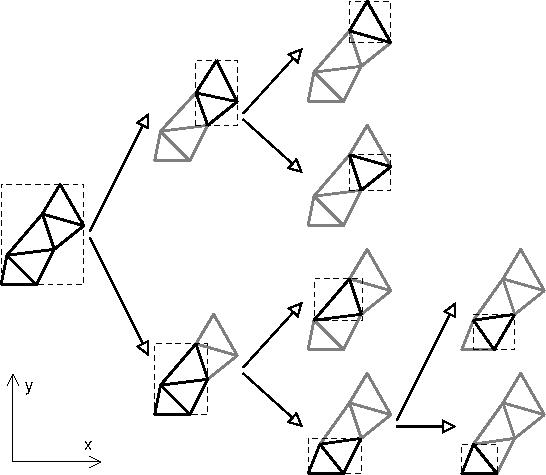
\includegraphics{figures/coll-volumes}}
\caption{Example tree of axis-aligned bounding boxes (AABBs).\label{collisionVolumes}}
\end{figure}

AABBs can very efficiently be tested for intersection. To determine whether two meshes are in
contact, the boxes at the roots of their AABB trees are tested against each other. If the boxes
intersect, all four pairings of their immediate children are tested. This procedure continues
recursively as long as the boxes intersect. At the leaves of the tree, the actual triangles are
tested for intersection.

\subsection{Finding the time of contact\label{findingContactTime}}

This collision detection algorithm returns nothing if meshes are separated merely by a very small
distance. Thus it is likely that bodies which were separate in one time step are suddenly found
to have interpenetrated in the next. There are elaborate solutions which predict the time of
impact using proximity detection and the bodies' velocities. I take a simpler approach: if, at
some time, meshes have penetrated beyond some tolerance threshold, the current simulation step
is discarded and retried using a smaller step length.

Retrying a step is quite expensive, so it is desirable to find the time of first contact with very
few retries. The depth of penetration can usually be estimated from the collision geometry, and
the velocities of the bodies are known from the simulation. Hence I can use the Newton-Raphson
algorithm~\cite{NRinC} for root finding (see figure~\ref{collisionTime}) to make a good guess at
the next step size. This method converges very rapidly in most cases, but occasionally it is
unstable, so my program resorts to binary search~\cite{Sedgewick:83} if the results of
Newton-Raphson seem erratic.

\begin{figure}
\psfrag{frag:0}{$0$}
\psfrag{frag:delta}{$-\delta$}
\psfrag{frag:t}{$t$}
\psfrag{frag:h}{$t+h$}
\psfrag{frag:hprime}{$t+h'$}
\centerline{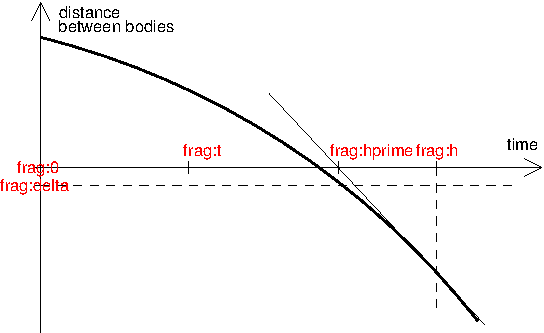
\includegraphics{figures/coll-time}}
\caption{Estimating a new step length $h'$ after penetration occurred when using step length $h$.
    The iteration stops when the penetration depth lies within the tolerance $\delta$.
    \label{collisionTime}}
\end{figure}

\subsection{Types of contact}

We are now in a state where the polygon meshes are in non-penetrative contact, i.e.\ there is some
intersection between their surfaces, but the intersection of their volumes is very small or zero.
Between polyhedral bodies we can identify several basic types of contact, two of which~--
\emph{vertex/face} and \emph{edge/edge} contact~-- are shown in figure~\ref{contacts1Figure}.

There are some more basic types of contact, like vertex/vertex contacts, but these occur only in
corner cases and can be approximated by other types of contact. Much more common is to have
several basic contacts occurring simultaneously, as shown in figure~\ref{contacts2Figure}. Bodies
may be concave, therefore the set of simultaneous contacts can become quite complicated. I would
like to claim that it is nevertheless possible to decompose an arbitrary collision geometry into
vertex/face and edge/edge contacts; however, I have not yet succeeded in backing up this claim
with a proof or in finding any research literature on this question.

\begin{figure}
\centerline{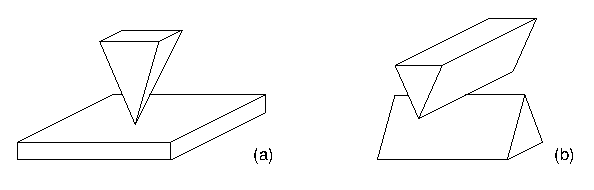
\includegraphics{figures/contacts1}}
\caption{Two basic types of polyhedral contact: \emph{(a)}~vertex/face, \emph{(b)}~edge/edge.
    \label{contacts1Figure}}
\end{figure}

\begin{figure}
\centerline{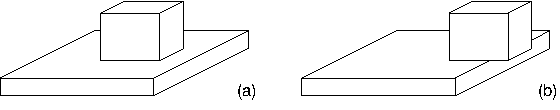
\includegraphics{figures/contacts2}}
\caption{Two examples of composite contacts between polyhedral bodies:
    \emph{(a)}~four vertex/face contacts (one for each corner on the upper cube's bottom face),
    \emph{(b)}~two vertex/face and two edge/edge contacts.
    \label{contacts2Figure}}
\end{figure}

Lacking a general algorithm to decompose contacts, my simulation only checks whether exactly one
vertex/face contact or one edge/edge contact is present (this can be done quite easily). If the
geometry does not match either, it is approximated by a single vertex/face contact. This
approximation can cause unrealistic behaviour in some cases, but I have not found it to be a
problem in practise.


\section{Collision and contact handling\label{collisionHandling}}

\subsection{Overview}

In all parts of the simulation discussed up to and including section~\ref{articulatedBodies}, the
acceleration was a continuous function of time; but collisions introduce discontinuities. These
discontinuities occur at the instant of first contact, and section~\ref{findingContactTime}
explained how to determine this point in time. I shall now consider the simulation state only at
this time of contact.

Let us distinguish two cases of contact between bodies: resting contact and colliding contact.
A book lying on a table is in resting contact with the surface: their relative velocity is zero,
but the desk exerts a force on the book to prevent it from penetrating into the surface.
Colliding contact is given for example between the ground and a ball bouncing off it. In reality,
the ball stays in contact with the ground for a finite length of time, during which it is
deformed and experiences a finite force accelerating it upwards. In our simulation, however, we
are working with rigid bodies which cannot be deformed, so we want the collision to happen
instantaneously in the moment when the ball touches the ground. One way of looking at this is as
an infinitely strong force acting over an infinitely short time, but a more useful representation
is in terms of an impulse which directly affects the momenta of the bodies.

Creating a simulation involving contacts is generally seen as a difficult task.
Baraff~\cite{BaraffWitkin:97} derives equations to handle collisions, and outlines (with a number
of errors) a way of handling resting contact. Unfortunately his collision handling does not work
in combination with constraints, and his resting contact computation relies on a complicated and
uncommon numerical routine. In this project, a new method of handling contacts is developed, which
is simpler to implement, more powerful, and works perfectly together with constraints like those
required for articulated bodies.


\subsection{Resting contact\label{restingContact}}

Bodies in resting contact exert equal and opposite forces on each other so that they do not
interpenetrate. This force must exactly balance the outside force, otherwise they will accelerate
apart. The direction of this force is perpendicular to the plane of contact; in the vertex/face
case, this is just the plane of the face polygon. In the edge/edge case, the plane goes
through the point of contact and is spanned by the directions of the two edges involved.
There is only one special case to be handled separately, namely when the two edges are parallel.

Note that we are not trying to simulate friction at this point. The force in the direction of the
contact plane normal merely stops interpenetration~-- if one were to push the book over the
horizontal table surface, it would glide without slowing down. Despite the movement, this contact
is resting because the relative velocity is parallel to the contact plane.

How do we now compute this contact force in an arbitrary system, where there may be objects stacked
on top of each other, different forces and torques acting, and so on? We can employ a constraint
function like in section~\ref{constraints}. For a vertex/face contact, let the value of this
function $c$ be the distance of the vertex point from the plane, being negative on
one side and positive on the other; for an edge/edge contact, the value is the distance between the
two straight lines. In contact, this distance is zero. In resting contact we also have
$\dot{c} = 0$. The function becomes interesting when we consider its second
derivative, $\ddot{c}$. If positive values of $c$ represent legal states (in which the
bodies are touching or separate), we can enforce the non-penetration constraint by requiring
\begin{equation} \label{constrInequality}
\ddot{c} \ge 0.
\end{equation}

More exactly, if it is the case that $\ddot{c} < 0$, we need to apply forces and torques
to the bodies such that afterwards we have $\ddot{c} = 0$. But when
$\ddot{c} \ge 0$, no force is applied (otherwise we would be glueing the book to the
table). But how do we solve this inequality in practise? At this point we diverge from Baraff's
method~\cite{BaraffWitkin:97}, who expresses equation~\ref{constrInequality} and additional
side conditions as a ``quadratic program'' and uses a specialized numerical solver.

Let us take a much simpler approach and pretend for now that equation~\ref{constrInequality}
contained an equals sign. Then this is a constraint like any other, which we can satisfy by using
the Lagrange multiplier method of section~\ref{constraints}. Moreover, if there are multiple
points of resting contact in the system, and also `real' constraints like joints between bodies,
we can solve all of these simultaneously without having to think twice.

However, having solved equation~\ref{lagrangeEquation} for \ve{\lambda}, we need to take care.
Observe equation~\ref{lagrangeSolution}, in which the constraint forces are computed:
\begin{equation}
\ve{\Phi}_c = \m{J}^T\ve{\lambda} = \sum_{i=1}^{m} (\ve{J}_i)^T \lambda_i
\end{equation}
Since each row of \m{J} is generated by a particular constraint, and the $i$th row of \m{J} is
scaled with component $\lambda_i$ of \ve{\lambda} in the linear combination of constraint forces,
we can say that each each component $i$ of \ve{\lambda} specifies the `amount' of constraint $i$
to apply to the system. Moreover, a positive value of the $\lambda_i$ component generates
forces and torques which push the bodies apart, while a negative value pulls them together (the
opposite sign convention is equivalent, but one convention must be used consistently). It is such
a negative $\lambda_i$ that we must avoid.

This gives us a basis for an algorithm which turns equation~\ref{constrInequality} back into what
it actually is~-- an inequality: set up constraint functions for all contact points, and solve the
system of linear equations for the Lagrange multiplier \ve{\lambda}. In this vector, find all
components relating to inequality constraints whose value is negative. (Equality constraints
are left untouched whatever their \ve{\lambda} component value is.)
If there are none, calculate $\m{J}^T\ve{\lambda}$ and add the forces and torques to the system~--
then we are done. If there are negative components, completely discard the constraints to which
they belong (since the bodies are accelerating away from each other in this point, the contact
will break in the next time step), then repeat the solving for \ve{\lambda} with the reduced set
of constraints. The process may take several iterations before terminating, but always terminates
because in each iteration we either reduce the number of active constraints or exit.

I have not yet been successful in proving this algorithm correct, but despite extensive pondering
I have not found any examples in which it fails either.

\subsection{Colliding contact\label{collidingContact}}

While points of resting contact had the property that $\dot{c} = 0$, colliding contact is
characterized by $\dot{c} < 0$. (If $\dot{c} > 0$ then the bodies are separating.
Such a contact can be ignored for now, but we cannot fully discard it, as explained
below.) The bodies' linear and angular momenta must be modified instantaneously to satisfy
$\dot{c}' \ge 0$, otherwise the bodies will interpenetrate in the next time step.

Physically, this operation is expressed in terms of an \emph{impulse}. An impulse \ve{u} has the
same dimensions as linear momentum \ve{p} (kg\,m/s) and is directly added to the momentum of the
body to which it is applied: $\ve{p}' = \ve{p} + \ve{u}$. If the impulse is applied at the point
$\ve{s}$, and \ve{r} is the body's centre of mass, it also changes the angular momentum to
$\ve{L}' = \ve{L} + (\ve{s} - \ve{r})\times\ve{u}$. This behaviour is analogous to that of a
force.

A collision between two bodies must conserve the total momentum of the system~\cite{Feynman:63}.
This implies that the impulses acting on the bodies at a point of collision must be equal and
opposite. However, the collision need not necessarily conserve energy. A collision which does
conserve energy is called \emph{elastic} or \emph{fully elastic}, and may be given for example
by an ideal rubber ball which, when dropped, bounces up to exactly the same height as it was
dropped from. At the other extreme, an \emph{inelastic} collision is one which reduces the energy
of the system as much as possible~-- the bodies do not `bounce apart' again.

Most real collisions are somewhere in between, depending on the materials of the colliding
objects. The elasticity is a scalar $0 \le \varepsilon \le 1$, where $\varepsilon = 0$ indicates
an inelastic collision, and $\varepsilon = 1$ full elasticity\footnote{Setting $\varepsilon > 1$
yields amusing results.}.

How do we now find the impulses we need to apply to the colliding bodies, and how do we
simultaneously handle constraints? Once again we can use a Lagrange multiplier method, but a new
equation must be derived which operates on impulses rather than on forces.

Set up a vector \ve{c} of concatenated constraint functions including all equality constraints
and all points of colliding contact. Points of resting contact and separating contacts must
not be included. Now for all points $i$ of colliding contact we have $\dot{c}_i < 0$.
Remember that this value is the relative velocity of the bodies in the point of contact,
projected onto the normal of the contact plane. Then the relative velocity $\dot{c}_i'$ after
the collision is given by $\dot{c}_i' = -\varepsilon_i \dot{c}_i$. The components of the relative
velocity parallel to the contact plain remain unchanged.

Assume for convenience that the first $m$ components of \ve{c} come from equality constraints, and
that the remaining $k$ components are due to inequalities.
Then $\dot{\ve{c}}'$ is the required value of $\dot{\ve{c}}$ after the collision:
\begin{equation}
\dot{\ve{c}}' = \left[\begin{array}[m]{c}
    \left. \begin{array}{c} 0 \\\vdots\\ 0 \end{array} \right\} m \\
    -\varepsilon_1 \dot{\ve{c}}_{m+1} \\\vdots\\
    -\varepsilon_k \dot{\ve{c}}_{m+k}
    \end{array}\right]
\end{equation}
i.e.\ we require all equalities to be satisfied, and all inequalities to have `bounced' by the
right amount. We can rewrite this as $\dot{\ve{c}}' = \dot{\ve{c}} - \m{E}\dot{\ve{c}}$, where
\m{E} is the diagonal $m+k \times m+k$ matrix
\begin{equation}
\m{E} = \left[ \begin{array}{cc}
    \begin{array}{ccc} 1 \\ & \ddots \\ && 1 \end{array} \\
    \underbrace{\quad\quad\quad\quad}_m &
    \begin{array}[t]{ccc} 1+\varepsilon_1 \\ & \ddots \\ && 1+\varepsilon_k \end{array}
    \end{array} \right]
\end{equation}

Let us now concatenate the linear and angular momenta of all $n$ bodies into a single vector
\ve{\Psi}, like we previously did for forces and torques (equation~\ref{PhiVector}):
\begin{equation} \label{PsiVector}
\ve{\Psi} = \left[\begin{array}{c}
    \ve{p}_1 \\ \ve{L}_1 \\ \vdots \\ \ve{p}_n \\ \ve{L}_n \end{array}\right]
\end{equation}

From the definition of $\m{M}^{-1}$ (equation~\ref{massInertiaTensor}) we can deduce that
$\dot{\ve{x}} = \m{M}^{-1}\ve{\Psi}$. We are seeking a vector $\ve{\Psi}_c$ which, when
added to $\ve{\Psi}$, causes the constraints to return the value $\dot{\ve{c}}'$:
\begin{equation} \label{cDotPrime}
\dot{\ve{c}} = \m{J}\dot{\ve{x}} = \m{J}\m{M}^{-1}\ve{\Psi} \quad\Longrightarrow\quad
    \dot{\ve{c}}' = \m{J}\m{M}^{-1}(\ve{\Psi} + \ve{\Psi}_c)
\end{equation}
(cf.\ equation~\ref{cDotAndCDDot}).
It turns out\footnote{The argument is analogous to the derivation of the force vector in terms of
Lagrange multipliers; see~\cite{BaraffWitkin:97} for details.} that this vector can be written as
$\ve{\Psi}_c = \m{J}^T\ve{\lambda}$ for some $m+k$-row vector \ve{\lambda}. Substituting the
previously defined expressions into equation~\ref{cDotPrime}:
\begin{eqnarray}
\dot{\ve{c}}' &=& \m{J}\m{M}^{-1}(\ve{\Psi} + \m{J}^T\ve{\lambda}) \nonumber\\
\dot{\ve{c}} - \m{E}\dot{\ve{c}} &=&
    \m{J}\m{M}^{-1}\ve{\Psi} + \m{J}\m{M}^{-1}\m{J}^T\ve{\lambda} \nonumber\\
\m{J}\m{M}^{-1}\ve{\Psi} - \m{E}\m{J}\m{M}^{-1}\ve{\Psi} & = &
    \m{J}\m{M}^{-1}\ve{\Psi} + \m{J}\m{M}^{-1}\m{J}^T\ve{\lambda} \nonumber\\
-\m{J}\m{M}^{-1}\m{J}^T\ve{\lambda} &=& \m{E}\m{J}\m{M}^{-1}\ve{\Psi} \label{collisionLagrange}
\end{eqnarray}

All variables in equation~\ref{collisionLagrange} are known except for \ve{\lambda}, so this is
just a system of linear equations which we can solve for \ve{\lambda}. The resulting vector
$\ve{\Psi}_c = \m{J}^T\ve{\lambda}$ of impulses can be directly added to the rigid bodies' momenta.

We are not quite finished yet. Having modified the bodies' momenta, the state of other contact
points in the system may have changed. While the previously colliding contacts will have
turned into resting or separating contacts, other (previously unconsidered) contacts may now
be colliding! Thus we must repeat the whole process described in this section, ignoring the
previously colliding points, and considering the new ones instead. If there are no new colliding
contacts, we have finished.

The bad news is that this algorithm is not guaranteed to terminate~-- indeed
figure~\ref{contacts3Figure} shows an example in which it will run indefinitely. An easy way of
solving this problem is by not allowing $\varepsilon$ to be too close to 1; then if a loop
occurs, the system will eventually run out of energy and return to a resting contact.

\begin{figure}
\centerline{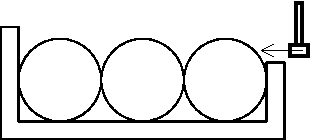
\includegraphics{figures/contacts3}}
\caption{Fully elastic spheres are packed tightly in a rigid box, with no space between them or at
    either end. When one is tapped horizontally with a hammer, the impulse travels up and down the
    chain forever, always being reflected at the walls of the box.\label{contacts3Figure}}
\end{figure}


\subsection{Generalized collisions\label{generalizedCollisions}}

In section~\ref{angleLimitation} I mentioned that the simulation still needed a way of limiting
the range of valid angles for a joint of an articulated body. I could not find any literature
explaining how one might realize such a constraint, but I was very excited to notice one day that
I already had all the tools in hand, and merely needed to combine them.

An angle limitation is simply another type of inequality constraint. Usually two constraints are
required for each axis about which rotation is possible:
\begin{eqnarray}
c_1 & = & \mbox{\textit{current angle}} - \mbox{\textit{minimum angle}} \nonumber\\
c_2 & = & \mbox{\textit{maximum angle}} - \mbox{\textit{current angle}} \label{genCollIneq}
\end{eqnarray}

The two inequalities $c_1 \ge 0$ and $c_2 \ge 0$ then require the current angle to always stay
within the range bracketed by the minimum and the maximum. Once $c_1$ and $c_2$ have been
formulated in an appropriate way, these inequalities can be given directly to the algorithms
for resting and colliding contact, alongside any other constraints generated by meshes in contact
or by joints. These algorithms will ensure that all constraints are satisfied simultaneously
(irrespective of their origin), and the result actually behaves just as expected!

The continuation of the good news is that I have already given a suitable formula to determine
the current angle of rotation about a particular axis in equation~\ref{rotationConstraintEqn}
(section~\ref{rotationConstraints}). This formula can simply be reused for inequalities.

There is just one problem: it is fiendishly hard to visualize what a particular restriction on
a 3D rotation actually means. The best I could come up with is to imagine a 3D phase space in
which each coordinate is the angle of rotation about one of the limb's local (Cartesian) axes.
The set of valid rotations for one joint is then a subspace of some shape; despite the linear
look of inequalities~\ref{genCollIneq}, this space is generally not polyhedral; in fact it is
often not even compact. Maple cannot visualize such a solution space of inequalities, so I wrote
myself a little program for this task (figure~\ref{jointLimit}) and used it to set up the joint
limits for Alfred's skeleton.

\begin{figure}
\centerline{\scalebox{0.32}{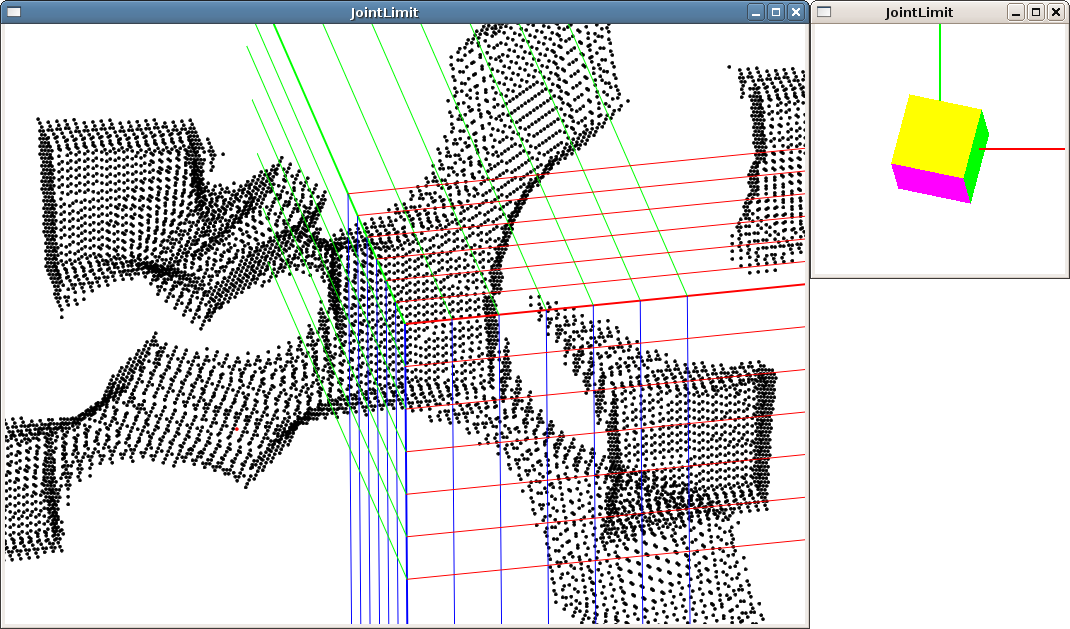
\includegraphics{figures/jointlimit}}}
\caption{Screenshot of a tool to visualize the solution space of simultaneous inequalities in
    three variables (here, the rotation about three different axes). If a point in the solution
    space is selected, the three angles of rotation corresponding to this point are applied to the
    cube on the right-hand side; this allows the inequalities to be adjusted to fit the desired
    set of rotations.\label{jointLimit}}
\end{figure}
